\cleardoublepage
\chapter{Long-read Sequencing}\label{ch: long_read_sequencing}

This chapter provides a detailed background into the lab workflow and bioinformatics pipelines developed during this PhD that were subsequently used to generate and analyse data from Pacific Bioscience (PacBio) SMRT sequencing (henceforth referred to as Iso-Seq) and Oxford Nanopore Technologies (ONT) nanopore cDNA sequencing in \textbf{Chapters 4-6}. 

\section{Pacific Biosciences: Isoform Sequencing}
\label{sec:pb_isoform_sequencing}

\subsection{Introduction}
Successful DNA polymerisation requires a high concentration of nucleotides for DNA polymerase processivity and accuracy. However, mimicking this in DNA sequencing results in a high background noise level, thereby reducing the sensitivity to detect base incorporation and fluorophore emission. Historically, “second-generation” sequencing technologies - such as that used in Illumina short-read RNA-Seq - have circumvented this issue by the step-wise addition, scan and wash of each set of labelled nucleotides, although at the expense of read lengths (as discussed in \cref{rnaseq_intro}). 

In 2013, PacBio pioneered the development of “third generation” long-read sequencing with the capability to generate substantially longer reads (reviewed in \cref{tab: longread_isoseqstudies}), due to its ability to mimic the natural, uninterrupted, processive DNA synthesis through three important innovations\cite{Eid2009}: 
\begin{enumerate}
	\item The creation of a circular template, SMRTbell (\cref{fig:Mechanism}\textbf{A}), which is enclosed with hairpin adapters at the ends of the insert, allowing uninterrupted DNA polymerisation \cite{Travers2010}.
	\item The sequencing of each polymerase-bound SMRTbell at the bottom of a nanometre-wide well (zero-mode waveguide - ZMW\nomenclature{ZMW}{Zero-mode waveguide})\cite{Levene2003} (\cref{fig:Mechanism}\textbf{B}). The nanoscale size of the ZMWs and reduced volume allow sensitive detection of a single nucleotide incorporation event against the high background of labelled nucleotides, achieving a high-signal-to-noise ratio. PacBio currently offers two sequencers, which primarily differ in the number of ZMWs that can be sequenced: Sequel I and Sequel II with 1 Million and 8 Million ZMWs, respectively.   
	\item The addition of phospholinked nucleotides, each labelled with a different colour fluorophore that corresponds to the four different bases (A, C, G and T), allows for natural and processive DNA synthesis\cite{Mccarthy2010} (\cref{fig:Mechanism}\textbf{C}). 
\end{enumerate}

\subsubsection{Mechanism}
Due to the circular nature of the SMRTbell template, the polymerase is able to continually read through the insert in an uninterrupted fashion multiple times (or “passes”), resulting in the generation of a continuous read (known as a “polymerase read”) (\cref{fig:Mechanism}\textbf{A}). By removing the hairpin-adapters that delineate the repeated insert sequence, this polymerase read is resolved to multiple reads (known as “subreads”), which are then merged to yield one high-quality and highly-accurate consensus read (known as a “circular consensus sequence” - CCS\nomenclature{CCS}{Circular consensus sequence}) (\cref{fig:Mechanism}\textbf{A}). The generation of these CCS reads can drastically improve a single-pass from 85\%, due to random sequencing error, to 99\% from alignment and correction of multiple subreads. Notably, the error rate is proportional to the number of “passes”, and is dependent on the polymerase lifetime and insert length\cite{Travers2010}. 

Unlike the short reads produced by standard Illumina-based RNA-Seq, PacBio Iso-Seq reads are not of a set length, but a range of lengths that is reflective of the library size and polymerase activity\cite{Ardui2018,Rhoads2015}. Previous chemistries preferentially sequenced molecules of a certain length, due to biased loading of SMRTbell templates; “Diffusion Loading” favoured shorter molecules\cite{Loomis2013}, whereas “Magbead Loading” allowed proportional loading of DNA templates to the concentration rather than length, but prevented sequencing of templates < 1kb. However, recent improvements in both technology and chemistry have alleviated this sequencing read-length bias \cite{Oikonomopoulos2020}.

\begin{figure}[!h]
	\centering
	\includegraphics[page=14,trim={0 5cm 0 0 },clip, scale = 0.7]{Figures/ProjectDevelopment_Figures.pdf}
	\captionsetup{width=0.95\textwidth}
	\caption[Pacific Biosciences single-molecule real-time sequencing technology]%
	{\textbf{Pacific Biosciences single-molecule real-time sequencing technology.} Shown is an overview of Pacific Biosciences single-molecule real-time sequencing technology (SMRT), which is able to generate long reads > 10kb by \textbf{(A)} enclosing the cDNA fragment of interest within a circular template (SMRTbell) to allow uninterrupted DNA polymerisation,  followed by the \textbf{(B)} sequencing of each SMRTbell with a bound polymerase at the bottom of ZMWs, enabling sensitive detection of polymerisation at the nucleotide level from \textbf{(C)} addition of phospholinked nucleotides with a differently-labelled fluorophore. ZMWs - Zero-mode waveguides.}
	\label{fig:Mechanism}
\end{figure}

\clearpage
\subsection{Lab workflow}
\label{chap:isoseq_labpipeline}
This section describes the lab workflow for PacBio Iso-Seq library preparation, which was subsequently implemented in the long-read sequencing experiments for global transcriptome and targeted profiling in \textbf{Chapters 4 and 6}, respectively. General methods pertaining to sample preparation, cDNA synthesis and amplification can be found in \cref{ch: general methodology}.

The Iso-Seq lab workflow for the global profiling of the transcriptome (\textbf{Chapter 4}), as outlined in \cref{fig:isoseq_wholelab_protocol}, involved three main steps: i) converting RNA to full-length cDNA using the Clontech SMARTer PCR cDNA synthesis kit (\cref{section:ch2_cDNA_synthesis_explanation}), ii) amplification (\cref{section:ch2_PCR_explanation}) and purification (\cref{section:ch2_AMPure_explanation}) of double-stranded cDNA, and iii) the preparation of SMRTbell libraries. 

The Iso-Seq lab workflow for the targeted profiling of the transcriptome (\textbf{Chapter 6}), outlined in \cref{fig:isoseq_targetedlab_protocol}, involved the incorporation of barcode sequences during cDNA synthesis to allow sample multiplexing and an additional step of target enrichment for the genes of interest.

\vspace{3cm}
\begingroup
\parindent=0em
\etocsettocstyle{\rule{\linewidth}{\tocrulewidth}\vskip0.5\baselineskip}{\rule{\linewidth}{\tocrulewidth}}
\etocsetnexttocdepth{5}
\localtableofcontents 
\endgroup

\begin{figure}[htp]
	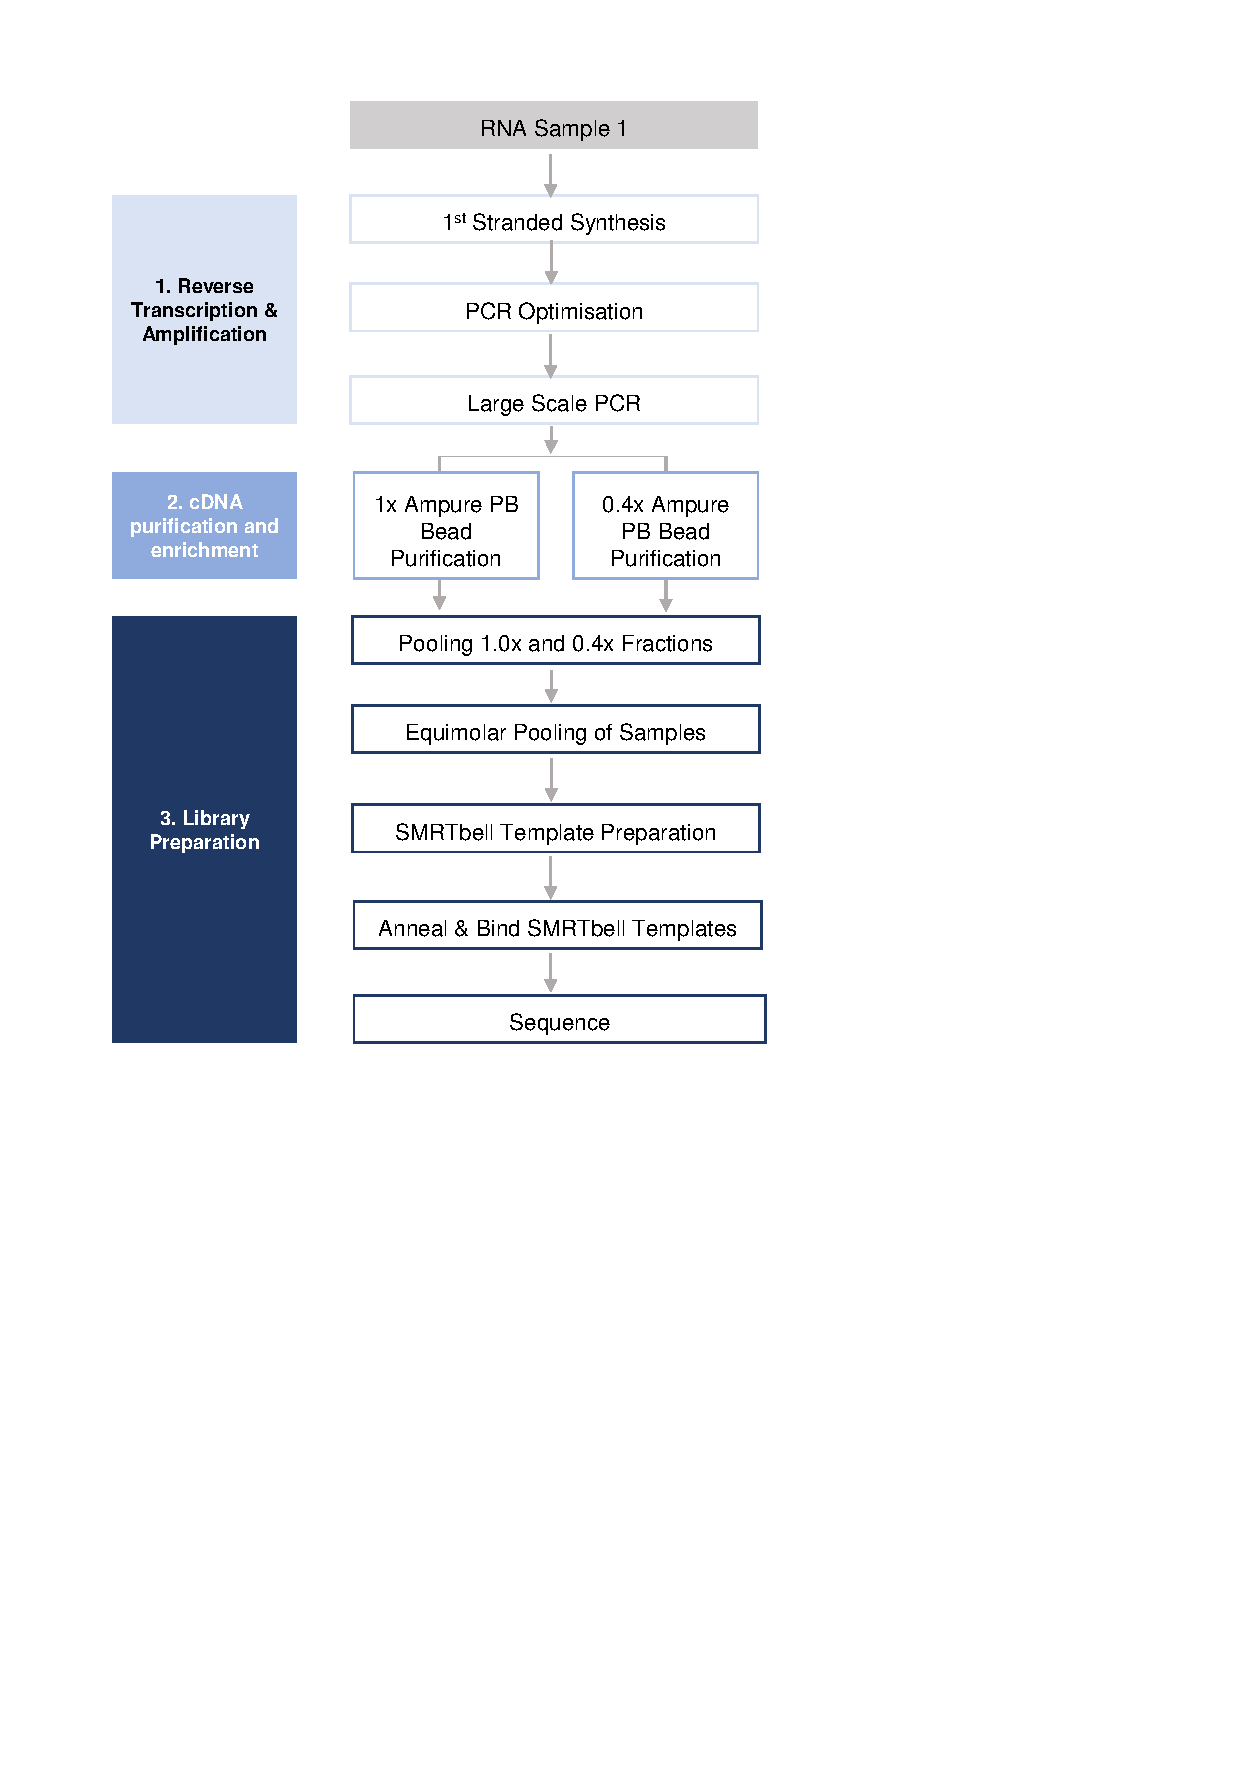
\includegraphics[page=1,trim={0 12cm 5cm 1cm},clip,scale = 1]{Figures/ProjectDevelopment_Figures.pdf}
	\captionsetup{width=0.95\textwidth}
	\caption[Iso-Seq lab workflow for global transcriptome profiling]%
	{\textbf{Iso-Seq lab workflow for global transcriptome profiling.} Shown is a flow diagram of the Iso-Seq lab workflow. Adapted from the official Iso-Seq protocol, it involves three main steps: 1) reverse transcription and amplification of cDNA (\cref{section:ch2_cDNA_synthesis_explanation}), 2) cDNA purification with AMPure beads (\cref{section:ch2_AMPure_explanation}), and 3) library preparation involving the ligation of SMRTbell templates, and binding of the primer and polymerase (\cref{section:ch2_smrtbelltemplate_explanation}). Due to the usage of newer chemistries, size selection was not performed.}
	\label{fig:isoseq_wholelab_protocol}
\end{figure}

\begin{figure}[]
	\begin{center}
		\includegraphics[page=2,trim={1cm 11cm 1cm 1cm},clip,scale = 0.8]{Figures/ProjectDevelopment_Figures.pdf}
	\end{center}
	\captionsetup{width=0.95\textwidth}
	\caption[Iso-Seq lab workflow for targeted profiling]%
	{\textbf{Iso-Seq lab workflow for targeted profiling.} Shown is a flow diagram of the Iso-Seq lab workflow for targeted profiling, which follows a similar workflow to that used in global transcriptome profiling (depicted in \cref{fig:isoseq_wholelab_protocol}), with the addition of a target cDNA capture step (boxed orange, described in \cref{section:ch2_targetcapture_explanation}) and the use of barcode sequences in cDNA synthesis (boxed green and denoted here as Barcode 1 and Barcode n) to allow sample multiplexing. The list of barcodes used can be found in \cref{tab:barcode_primers}.}
	\label{fig:isoseq_targetedlab_protocol}
\end{figure}

\clearpage
\subsubsection{PCR optimisation and DNA amplification}\label{ch: pcr_optimisation}
After cDNA synthesis, cDNA products were amplified using PCR to generate sufficient material for sequencing. To minimise PCR bias resulting in under- or over-representation of specific cDNA library sizes, the optimum number of PCR cycles for amplification was determined using the PrimeSTAR GXL DNA Polymerase (Clontech) (\cref{fig:pcr_optimisation_gel_eg}). This involved collecting 5$\mu$L PCR aliquots every two cycles (cycles 10, 12, 14, 16, 18 and 20) followed by the visualisation of cDNA products with ethidium bromide on a 1.5\% agarose gel. The optimum cycle number was determined by the cycle that generated sufficient amount of cDNA without compromising on the molecular weight, which is typically observed with PCR over-amplification of cDNA (\cref{fig:pcr_optimisation_gel_eg}). Large-scale PCR amplification was then subsequently performed using the optimum number of cycles, which is typically 14 cycles (as illustrated later in \cref{fig:isoseq_whole_bioresults} and \cref{fig:isoseq_targeted_pccresults}) . 

\begin{figure}[htp]
	\begin{center}
		\includegraphics[page=13,trim={1cm 24cm 10cm 1cm},clip,scale = 0.9]{Figures/ProjectDevelopment_Figures.pdf}
	\end{center}
	\captionsetup{width=0.95\textwidth}
	\caption[Example of an agarose gel for determining the optimum number of PCR cycles]%
	{\textbf{Example of an agarose gel for determining the optimum number of PCR cycles.} Shown is an agarose gel of human brain total RNA after first-strand cDNA synthesis and PCR amplification through cycles 8 to 18, with PCR aliquots collected every two cycles. In this example, 10 cycles were determined to be the optimum number for large-scale amplification. While the smear distribution from 8 and 10 cycles looked similar, 10 cycles showed a slightly stronger smear, thereby generating more material for downstream pooling. Cycles above 12 showed signs of over-amplification, which would result in biased sequencing representation. Figure and legend are adapted from Iso-Seq protocol.}
	\label{fig:pcr_optimisation_gel_eg}
\end{figure}


\subsubsection{AMPure bead purification} 
\label{section:ch2_ampurebead_pool} 
After large-scale amplification, the resulting PCR products were divided into two fractions for purification with either 0.4X or 1X AMPure PB beads (PacBio). DNA purification with 0.4X AMPure beads was essential to ensure enrichment of longer fragments for sequencing (as described in \cref{section:ch2_AMPure_explanation}). The quantity and size distribution of each fraction were then determined using the Qubit dsDNA High Sensitivity assay (Invitrogen) (\cref{section:ch2_qubit}) and Bioanalyzer assays on the 2100 Bioanalyzer (Agilent) (\cref{section:ch2_bioanalyzer}). The molarity of the two fractions were then calculated using \textbf{Equation \ref{eqn:isoseq_library_molarity}}, and equal molar quantities of the two fractions were subsequently pooled for library construction with the SMRTbell Template Prep Kit v1.0 (PacBio). 

\begin{equation}
	\label{eqn:isoseq_library_molarity}
	\frac{concentration(\frac{ng}{\mu L})\times 10^6}{660(\frac{g}{mol}) \times average\:library\:size\:in\:bp\mbox{*}} = concentration\;in\; nM
\end{equation}
* the average library size was determined by the start and end point of the cDNA smear on the BioAnalyzer

\subsubsection{Target capture using IDT probes} 
\label{section:ch2_targetcapture_explanation} 
Targeted profiling of the transcriptome was performed as part of the long-read sequencing experiments described in \textbf{Chapter 6}. This first involved equimolar pooling of uniquely-barcoded samples, followed by enrichment for target genes with a hybridisation-based capture approach (IDT). Through this approach, regions of interest within the library were captured (“hybridised”) using pre-designed, 5’ biotinylated, 120 nucleotide-long oligonucleotide baits (henceforth referred to as “probes”, \cref{fig:isoseq_targetcapture}\textbf{A}). Magnetic streptavidin beads were then used to isolate the hybridised library fragments for amplification (using Takara Hot-Start polymerase) and AMPure bead purification (outlined in \cref{fig:isoseq_targetcapture}\textbf{B}). After assessing the quality and quantity of the target cDNA with Qubit and Bioanalyzer assays, SMRTbell library preparation was proceeded according to manufacturer's protocol.  

%*Modifications to the protocol: waiting times at room temperature during hybridisation, lid heat temperatures, method of washing beads at room temperature; all modifications are incorporated from official IDT protocol, post amplification clean-up for consistency  

\myparagraph{Probe Designs}
Probes were designed to a selective panel of 20 AD-associated genes (henceforth referred to as “target genes”): \textit{Abca1, Abca7, Ank1, Apoe, App, Bin1, Cd33, Clu, Fus, Fyn, Mapt, Picalm, Ptk2b, Rhbdf2, Snca, Sorl1, Tardbp, Trem2, Trpa1, Vgf} - the relevance of these genes in AD pathogenesis are detailed later in \textbf{Chapter 6} (\cref{tab: TargetGenes_LitReview}). Two separate pools of equimolar probes were designed against the mouse (GRCm28/mm10) and human genome (GRCh37/hg19). While IDT provided a pre-designed set of probes to the exons of target genes (depicted in \cref{fig:target_probes_eg}\textbf{A}), the majority of exons were unnecessarily covered by contiguous probes, which can induce off-target binding and additional costs. Considering that previous targeted sequencing studies using the same hybridisation-based capture have achieved successful enrichment and sequencing with a few unique probes to the exonic region\cite{Sheynkman2020}, I manually assessed the list of probes for each target gene using the following criteria:
\begin{itemize}
	\item All of the exons must be covered by at least one probe.
	\item Probes should be spaced 300 - 500bp within each exon (equivalent to 0.2x – 0.3x tiling density). 
	\item Probes with the highest GC content (40 - 65\% GC content) and lowest number of blast hits were selected from the contiguous cluster. 
	\item Any probes covering the intronic regions were removed.
\end{itemize}
Examples of the initial set of probes provided by IDT and the final curated sets of probes after my filtering are illustrated in  \cref{fig:target_probes_eg}\textbf{B,C}. 

\begin{figure}[!h]
	\begin{center}
		\includegraphics[page=12,trim={0cm 6cm 0cm 1cm},clip,scale = 0.70]{Figures/ProjectDevelopment_Figures.pdf}
	\end{center}
	\captionsetup{width=0.95\textwidth}
	\caption[Lab workflow for hybridisation-based cDNA capture for targeted profiling]%
	{\textbf{Lab workflow for hybridisation-based cDNA capture for targeted profiling.} Shown is \textbf{(A)} a schematic figure of the target gene enrichment step involving hybridisation of cDNA with probes and blocking oligonucleotides (such as oligonucleotides complementary to the poly(A) tail and cDNA synthesis primers), followed by isolation with streptavidin beads. The addition of blocking oligonucleotides prevents non-specific binding, and subsequently increases capture rate and target gene sequencing coverage. \textbf{(B)} An overview of the lab workflow.}
	\label{fig:isoseq_targetcapture}
\end{figure}

\begin{landscape}
	\begin{figure}[!ht]
		\begin{center}
			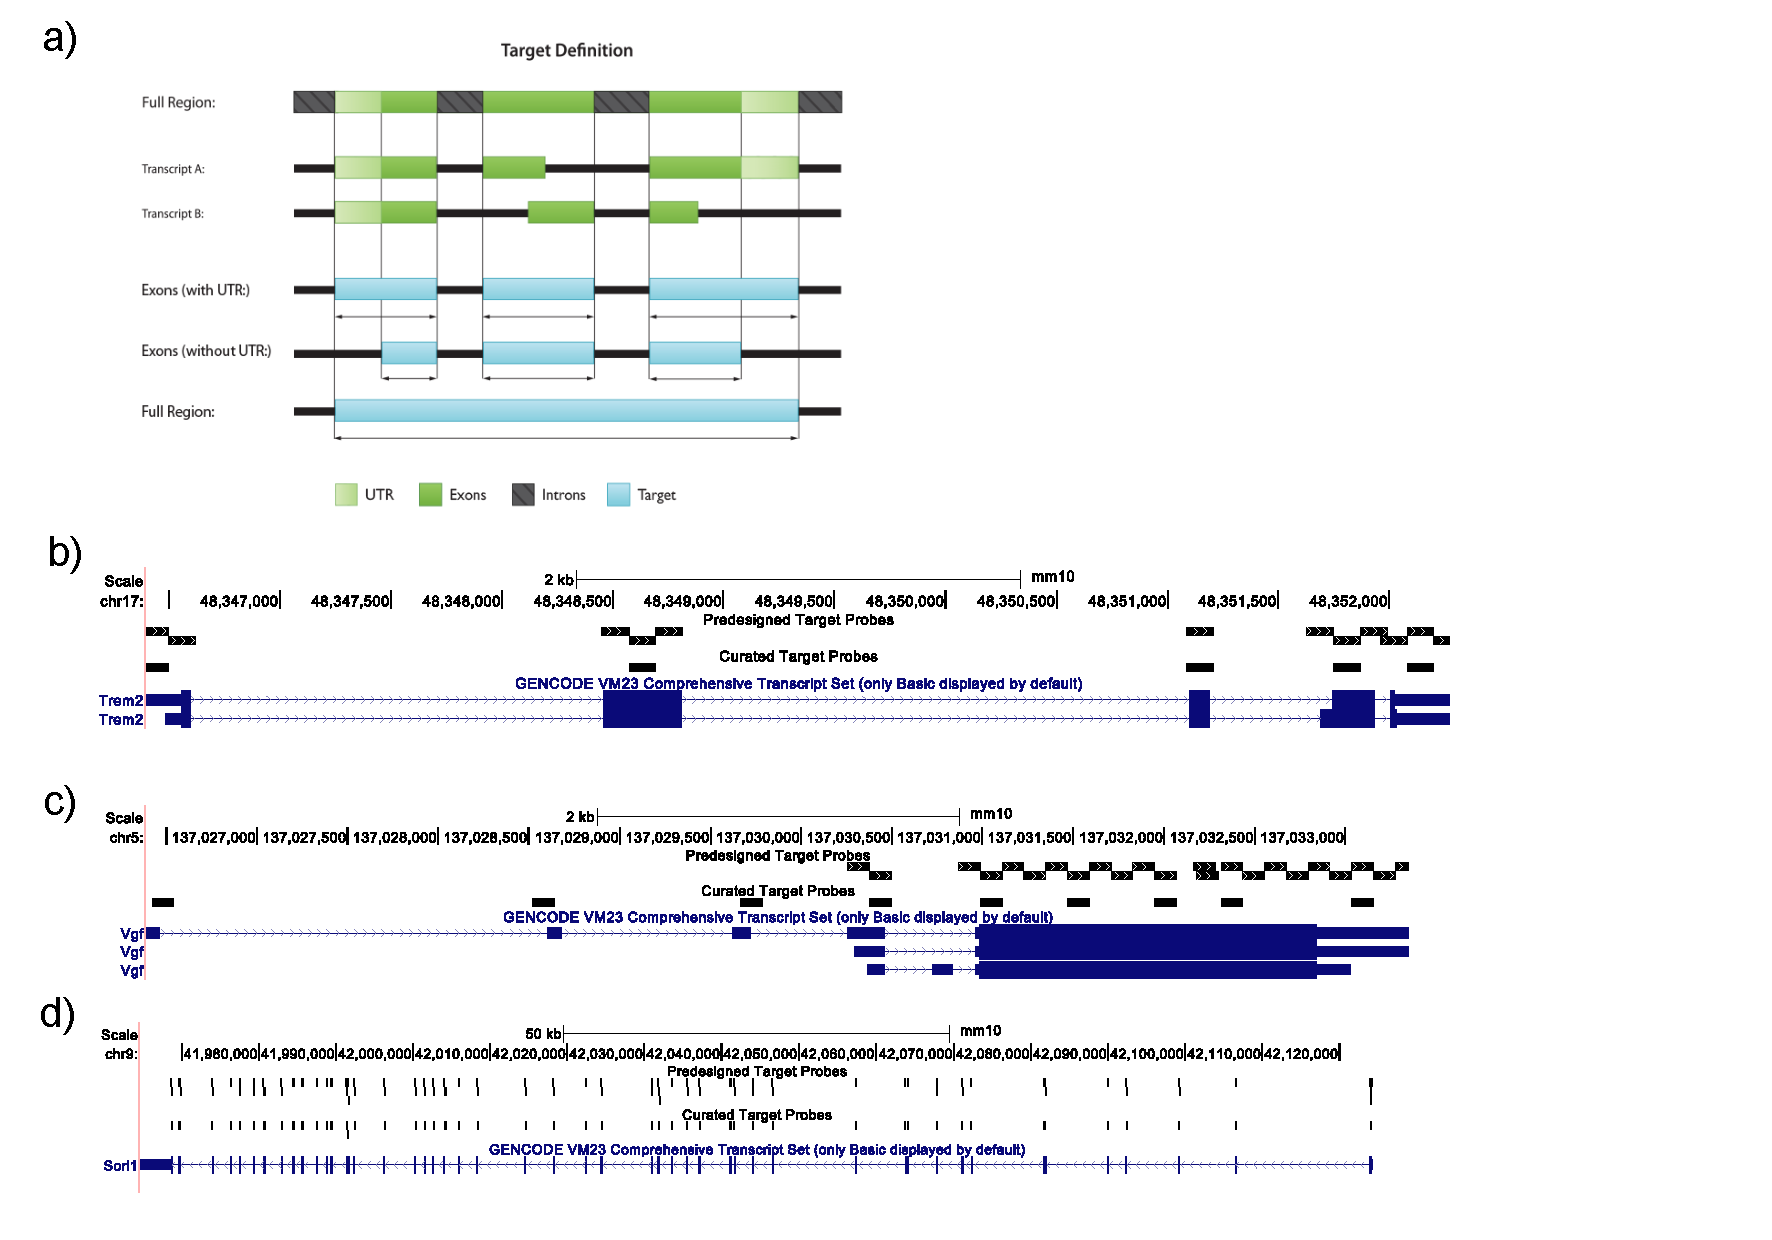
\includegraphics[page=1,trim={0cm 10cm 0cm 0cm},clip,scale = 0.90]{Figures/TargetProbes_Visualisation.pdf}
		\end{center}
		\captionsetup{width=1.5\textwidth}
		\caption[Manual curation of probes designed to 20 AD-associated target genes]%
		{\textbf{Manual curation of probes designed to 20 AD-associated target genes.} \textbf{(A)} Pre-designed set of probes were provided to “Exons (with UTR)” of target genes. Shown are UCSC genome browser tracks of pre-designed and curated probes to \textbf{(B)} \textit{Trem2}, and \textbf{(C)}\textit{Vgf} in the mouse genome (mm10). As shown, exons were unnecessarily covered by contiguous probes, which not only increase costs, but also induce off-target binding (referred in Figure B and C as “Pre-designed Target Probes”). Manual curation was therefore needed for each target gene (referred in Figure B and C as “Curated Target Probes”) to ensure that exons were covered with one probe for every 500bp. }
		\label{fig:target_probes_eg}
	\end{figure}
\end{landscape}

\subsubsection{Library preparation, primer annealing \& polymerase binding}
\label{section:ch2_smrtbelltemplate_explanation} 
After equimolar pooling of the two size fractions for global transcriptome profiling or multiple samples for targeted profiling (\cref{section:ch2_ampurebead_pool}), SMRTbell template preparation was performed with the SMRTbell Template Prep Kit v1.0 (PacBio). This first involved repairing DNA damage and polishing the ends of fragments (\cref{fig:isoseq_labworkflow}, Step 1, 2), which is essential for the generation of high-quality libraries of closed, continuous and circular SMRTbell templates. Abasic sites were filled-in, thymine dimers resolved, and deaminated cytosine alkylated. 3’ overhangs were removed, whereas 5’ overhangs were filled-in by T4 DNA Polymerase and phosphorylated by T4 PNK for ligation of blunt hairpin adapters. Following 1X AMPure bead purification of repaired dsDNA, hairpin adapters were ligated to the blunt ends for 24 hours (\cref{fig:isoseq_labworkflow}, Step 3). Any templates failing to ligate were removed with exonuclease III and VII (\cref{fig:isoseq_labworkflow}, Step 4). The repaired and ligated SMRTbell library was then purified with two rounds of 1X AMPure beads, and assessed for quality and quantity with Qubit and Bioanalyzer assays before proceeding to primer annealing and polymerase binding (\cref{fig:isoseq_labworkflow}, Step 5, 6). Of note, the primer and polymerase to template ratio was key to successful loading of SMRTbell templates into ZMWs for sequencing, and was dependent on the final library molarity (as determined using \textbf{Equation \ref{eqn:isoseq_library_molarity}}). 


\subsubsection{Loading and sequencing} 
\label{section:ch2_sequencing}
All Iso-Seq experiments in this thesis were performed on the PacBio Sequel 1M SMRT cell. Samples were processed using either the v3 chemistry (Diffusion Loading at 5pM with a 4-hour pre-extension and a 20-hour capture time) or v2.1 chemistry (Magbead Loading at 50pM with a 2-hour pre-extension and a 10-hour capture time). As suggested in the name, Diffusion Loading involves immobilising polymerase-bound SMRTbell templates to ZMW by diffusion, whereas Magbead loading uses paramagnetic beads (“Magbeads”) that roll across the ZMWs. Due to the different nature of loading, Diffusion Loading preferentially loads shorter transcripts, whereas Magbead Loading preferentially loads longer transcripts (> 1b). As a quality-control measure of loading and sequencing performance, a DNA internal control complex (PacBio) was added to each library before sequencing, the amount of which was dependent on the final library molarity. Mimicking SMRTbell templates, this internal control is composed of a 1966bp-insert with the SMRTbell adapters already ligated and the polymerase already bound.


\begin{figure}[!htp]
	\begin{center}
		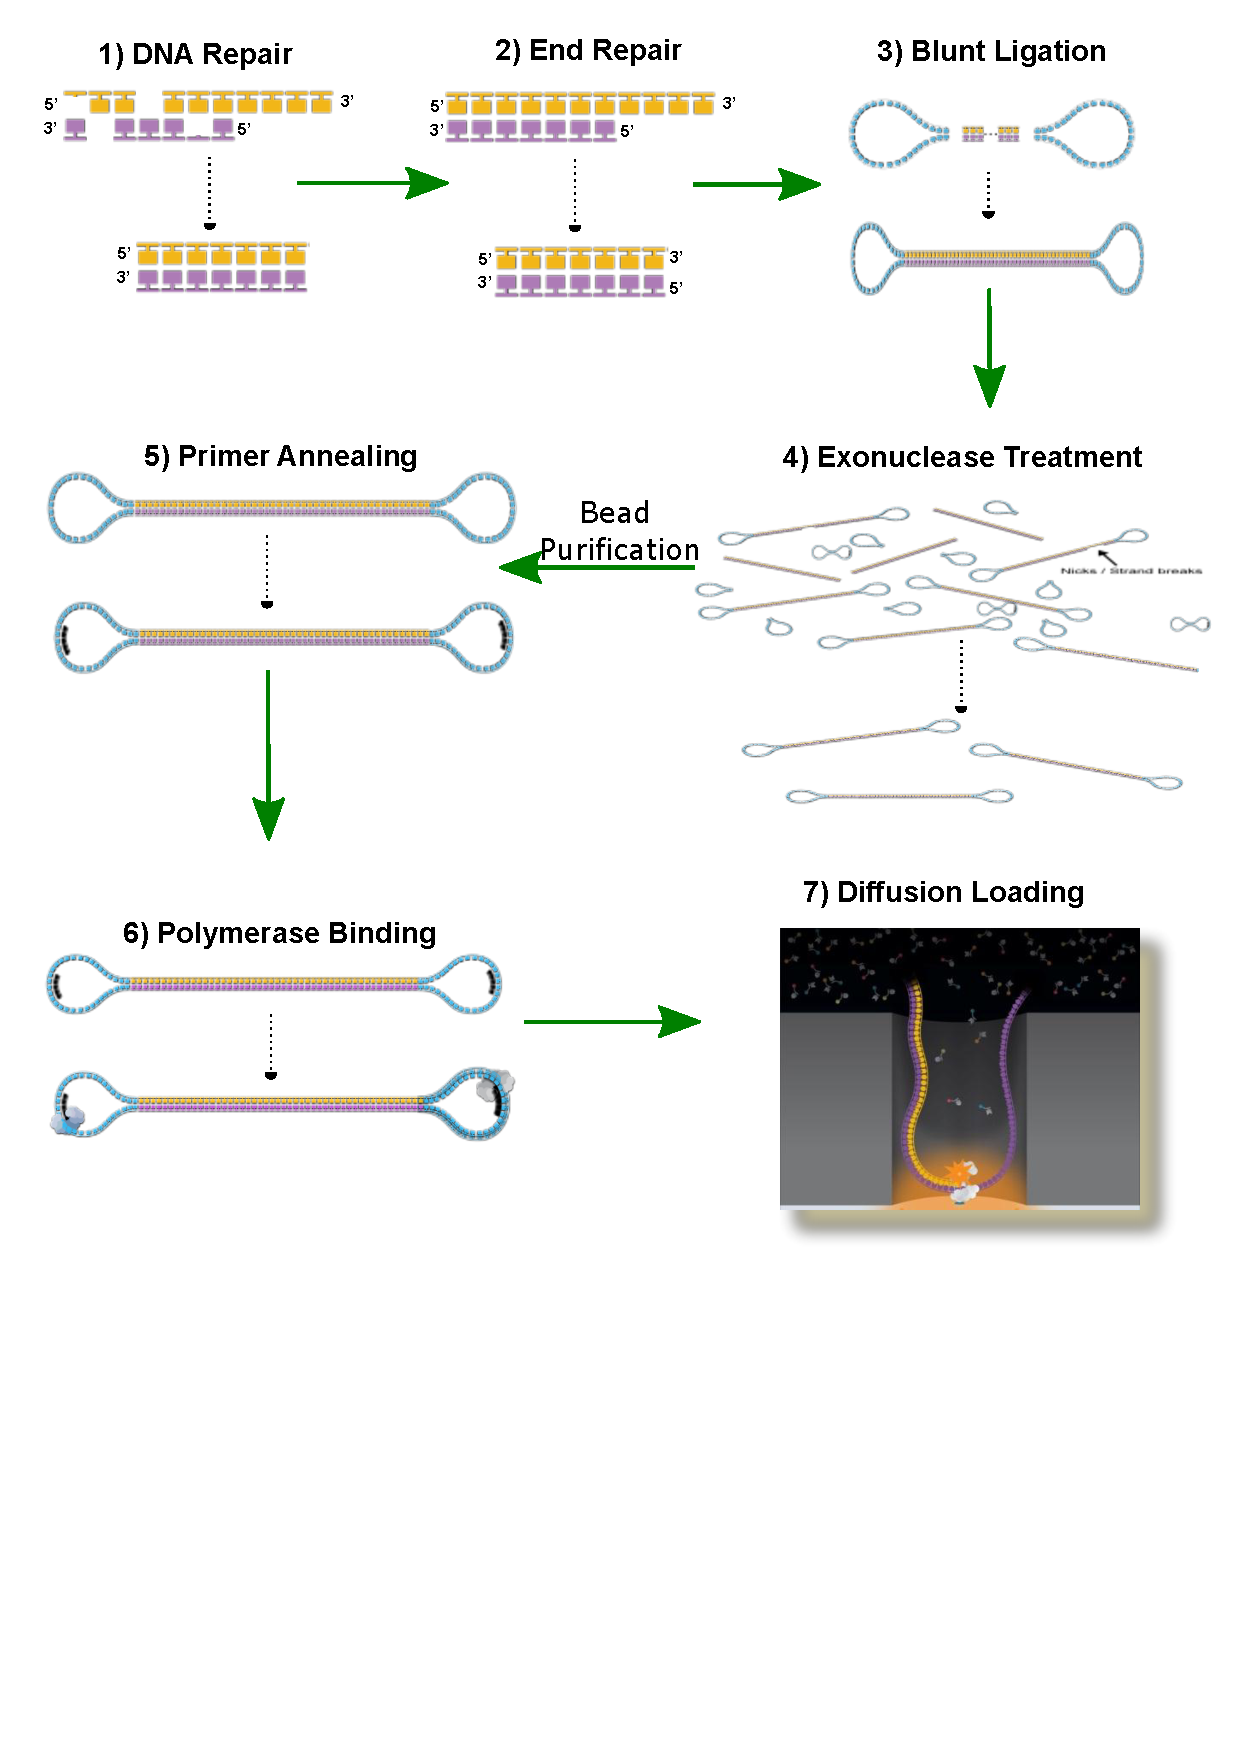
\includegraphics[page=1,trim={0cm 8cm 0cm 0cm},clip,scale = 0.70]{Figures/labwork_isoseq.pdf}
	\end{center}
	\captionsetup{width=0.95\textwidth,singlelinecheck=off}
	\caption[Detailed Iso-Seq lab workflow for SMRTbell library preparation]%
	{\textbf{Detailed Iso-Seq lab workflow for SMRTbell library preparation.} Shown is a flow diagram of the Iso-Seq lab workflow for library preparation:
		\begin{enumerate}
			\item Repair DNA by filling-in abasic sites, removing thymine dimers, oxidising guanines and deaminating cytosines. This is essential to ensure that there is a continuous sequence for uninterrupted polymerase processivity.
			\item Repair ends for blunt ligation with removal of 3' hangs and addition of 5' hangs by T4 DNA polymerase, which is required for blunt ligation of SMRTbell adapters. 
			\item Blunt Ligation by adding hairpin SMRTbell adapters to repaired ends.
			\item Exonuclease treatment to remove incomplete SMRTbell templates with Exonuclease III and IV to ensure optimal sequencing.
			\item Annealing of primers to both ends of the SMRTbell templates to initiate sequencing. 
			\item Binding of polymerase to both ends of the SMRTbell templates for efficient loading into ZMWs.
			\item Immobilisation of polymerase-bound SMRTbell templates to ZMW by diffusion.
			\\
		\end{enumerate} 
		Individual figures and legend are taken and adapted from “PacBio Sequel Library and Sequencing Preparation” presentation.
	}
	\label{fig:isoseq_labworkflow}
\end{figure}

\clearpage
\subsection{Run performance and quality metrics}
\label{sec: Isoseq_run_performance}
Suboptimal PacBio sequencing performance can result from various causes including potential issues with the instrument and sequencing reagents to poor library preparation and incorrect loading. The performance of a sequencing run can be assessed by the performance of the DNA internal control and various productivity metrics. 

\boldheader{DNA internal control} 
Sequencing metrics for the DNA internal control (described in \cref{section:ch2_sequencing}) is provided in several ways: i) the number of control reads, ii) the mean control polymerase read length, and iii) the proportion of sequence identity match between the control raw reads and the reference control (concordance). Short control read lengths and/or low control read counts are suggestive of issues with the PacBio instrument and consumables, while a low concordance value (< 0.84) indicates overloading of SMRT cells. Conversely, normal control sequencing metrics in a run with overall low yield indicate sample-specific issues. The expected sequencing metrics from a correctly prepared control in an optimal Iso-Seq sequencing run are documented in \cref{tab:control_Isoseqmetrics}. 

\vspace{1cm}
\begin{table}[!h]
    \setlength\tabcolsep{4pt} %reduced margin size in table
	\caption[Iso-Seq DNA internal control sequencing metrics]%
	{\textbf{Iso-Seq DNA internal control sequencing metrics.} Tabulated are the expected median values for the number of control reads (median count), the control polymerase read length (median length), and the identity match between control raw reads and reference sequence (median concordance). The expected values provided assume a sequencing run using the PacBio Sequel 1M SMRT cell with a 4-hour pre-extension and a 20-hour capture time. QR - Quantile range.}	\label{tab:control_Isoseqmetrics}
	
	\centering
	\begin{tabular}{@{}cccc@{}}
		\toprule
		Metrics         & Median count (QR)     & Median length (kb) (QR) & Median concordance (QR) \\ \midrule
		Expected values & 6900 (4000 - 10200) & 46.9 (41.5 – 52.5) & 0.862 (0.857 – 0.867)   \\ \bottomrule
	\end{tabular}
\end{table}


\boldheader{Productivity metrics} 
Productivity or loading metrics provide a measure of the number of ZMWs that generated a positive signal that was then translated into useful sequencing data. Each ZMW is classified as either: 
\begin{itemize}
	\item P0 (Productivity 0): no active sequencing polymerase complex with no signal. 
	\item P1 (Productivity 1): productive ZMWs with a high-quality (HQ)\nomenclature{HQ}{High-quality} sequence within read.
	\item P2 (Productivity 2): detectable signal but no HQ sequence detected, possibly due to overloading of multiple inserts with multiple polymerases.
\end{itemize}

An optimal sequencing run would achieve a total run yield of 20 - 30Gb with \textasciitilde70\% of ZWMs in P1 (positive signal), and 20 - 30\% ZMWs in P0 (empty ZMWs). A low P0 (< 20\%) indicates over-loading of polymerase-bound templates, resulting in shorter P1 polymerase reads and poor sequencing yield (noisy basecalling). Conversely, a high P0 (> 40\%) from under-loading would generate fewer P1 reads and result in a lower sequencing yield. A combination of high P0, low P1 and high P2 loading profiles indicates presence of contaminants (possibly from poor AMPure bead purification) that is interfering with productive polymerase activity. A good balance between P0, P1 and P2 is therefore key to achieving a good sequencing run with high yield and high-quality, long P1 polymerase reads. Multiple titrations of loading concentrations can be trialled to determine the optimum loading concentration essential for reaching this balance. 

\clearpage
\subsection{Bioinformatics pipeline} 
\label{section:isoseq_bioinformatics}
This section describes the bioinformatics pipeline that we established for analysing Iso-Seq data generated on the PacBio Sequel I following Iso-Seq library preparation (\textbf{Chapters 4 - 6}). 

The bioinformatics pipeline, as depicted in \cref{fig:isoseq_bioinformatics_Pipeline}, involves three main steps: i) the processing and filtering of raw reads to generate HQ, full-length transcripts using the PacBio \textit{IsoSeq3} suite \cite{Gordon2015}, ii) the alignment of HQ transcripts to the reference genome using \textit{Minimap2}\cite{Li2018}, and iii) the clustering and collapsing of mapped transcripts to unique, annotated isoforms using \textit{Cupcake}\cite{TsengCupcake} and \textit{SQANTI}\cite{Tardaguila2018}. Public annotations and short-read RNA-Seq data were used for validating Iso-Seq-derived isoforms. 

While raw Iso-Seq data can be processed using the PacBio SMRT Link Suite, a web-based end-to-end user interface, we developed an end-to-end command line that allowed simultaneous parallel processing of multiple samples and streamlining of the analysis after raw read processing. The choice of parameters and packages was guided by a separate analysis on external RNA spike-in controls (ERCC) that were sequenced within the same runs (described in \cref{section:ch2_ERCC_explanation}). 

\begingroup
\parindent=0em
\etocsettocstyle{\rule{\linewidth}{\tocrulewidth}\vskip0.5\baselineskip}{\rule{\linewidth}{\tocrulewidth}}
\etocsetnexttocdepth{5}
\localtableofcontents 
\endgroup


\begin{figure}[]
	\centering
	\vspace{20pt}
	\includegraphics[page=17,trim={0 6cm 0 0},clip,scale = 0.8]{Figures/ProjectDevelopment_Figures.pdf}
	\captionsetup{width=0.95\textwidth}
	\caption[Iso-Seq bioinformatics pipeline]%
	{\textbf{Iso-Seq bioinformatics pipeline.} Shown is an overview of the Iso-Seq bioinformatics pipeline used in this thesis, which involves three main steps: i) processing and filtering of raw reads into high-quality, full-length transcripts using \textit{IsoSeq3}, ii) alignment of HQ transcripts to the reference genome using \textit{Minimap2} and iii) collapsing of mapped transcripts to unique, annotated isoforms using \textit{Cupcake} and \textit{SQANTI}. HQ - High-quality.}
	\label{fig:isoseq_bioinformatics_Pipeline}
\end{figure}

\clearpage
\subsubsection{Processing of Iso-Seq raw reads}
\label{section: Isoseq_rawprocessing}
In response to the much higher experimental throughput of the PacBio Sequel compared to the older PacBio RSII sequencer, the official PacBio bioinformatics suite for processing Iso-Seq reads (henceforth referred to as \textit{Iso-Seq3}) has been revised multiple times over the course of this PhD. Each subsequent version delivered a reduction in runtime coupled with an improvement in sensitivity and specificity to recover transcripts and reduce artefacts. A particularly noteworthy development was the forgoing of non-FL reads or RNA-Seq short-reads for error correction, due to the high throughput and subsequent generation of high-quality, accurate Iso-Seq reads. 

Despite multiple major updates to \textit{Iso-Seq3}, the core principles and processing steps have remained the same (depicted in \cref{fig:isoseq3_tool}), namely: i) the generation of CCS reads from each sequencing ZMW, ii) the identification of full-length reads with the removal of cDNA primers and poly(A) tails, and iii) the grouping of full-length reads derived from the same transcript. 

\boldheader{Generation of CCS reads with \textit{CCS}}
Raw Iso-Seq subreads from each productive ZMW were processed to generate one representative circular consensus read (\cref{fig:isoseq3_tool}\textbf{A,B}) using \textit{CCS} (v5.0.0) with the following parameters: 
\begin{itemize}
	\item minimum number of full “passes” for a ZMW to be considered. A full pass is defined by the presence of both SMRT adapters at both ends (default: 3 passes).
	\item minimum predicted read accuracy across all subreads (default: 99\%).
	\item minimum and maximum length of subreads to generate a CCS (default: 10 and 21000 bases, respectively).
	\item quality of subreads predicted by the CCS model (default: -3.5 Z-score), and proportion of total subreads meeting the quality score (default: > 30\%).
\end{itemize}

%Across literature and PacBio scientific community, different parameter settings were recommended, particularly with \textit{number of full passes} and \textit{minimum base accuracy}, which had the greatest effect on the number of CCS reads generated for downstream analyses. Taking a subset of raw data from 10 randomised samples, a range of values across these two parameters were tested. CCS were then classified to full-length (FL, determined by the presence of 3'/5' primers and poly-A tail) and non-full-length (NFL) reads. 

\boldheader{Removal of primers and barcodes with \textit{lima}}
After the successful generation of CCS reads, cDNA primers were identified and removed using \textit{lima} (v2.0.0) to generate full-length (FL) reads (\cref{fig:isoseq3_tool}\textbf{C}). Additional barcode sequences were also removed for targeted sequencing experiments to perform sample demultiplexing. Sequences were then orientated from 5’ to 3’, and any reads with unwanted combinations were removed. Of note, the ratio of recovered FL reads to CCS reads varies on the insert transcript size, but a good sequencing library with a distribution of 1kb - 3kb should recover 60 - 70\% of CCS reads as FL reads.   

\boldheader{Trimming of poly(A) tails and concatemer removal with \textit{Iso-Seq Refine}}
FL reads were further refined by the trimming of poly(A) tails (with a minimum length of 20 adenosine bases). Artificial concatemers were then removed to ensure a library of full-length non-chimeric (FLNC\nomenclature{FLNC}{Full-length non-chimeric}) reads (\cref{fig:isoseq3_tool}\textbf{D}). Of note, artificial concatemers are cDNA sequences with internal runs of poly(A) and poly(T) sequences that were generated from using insufficient amount of blunt adapters during library preparation. The occurrence of these artefacts should be low (< 0.5\%) in a standard library preparation, and the number of FLNC reads and FL reads should be similar. Any significant loss of reads at this stage implicates issues with SMRTbell library preparation.

\boldheader{Grouping of reads into transcripts with \textit{Iso-Seq Cluster}}
Using an iterative isoform-clustering algorithm, two or more FLNC reads were then grouped and considered to be the same transcript if they: 
\begin{itemize}
	\item differed < 100bp on the 5’ end*. 
	\item differed < 30bp on the 3’ end. 
	\item did not contain internal gaps with > 10bp.
\end{itemize}
* Greater leeway was given to the 5' end than the 3' end to account for 5' RNA degradation.

A minimum of two FLNC reads was required for clustering with the longest read chosen as the representative transcript, and any unique FLNC reads failing to cluster were discarded (\cref{fig:isoseq3_tool}\textbf{E}). Transcripts generated from the \textit{Iso-Seq Cluster} were therefore high-quality with a consensus accuracy $\geq$ 99\% and a minimum of two FLNC read support (\cref{fig:isoseq3_tool}\textbf{F}). 

\begin{figure}[htp]
	\centering
	\includegraphics[page=18,trim={0 8cm 0 0},clip,scale = 0.8]{Figures/ProjectDevelopment_Figures.pdf}
	\captionsetup{width=0.95\textwidth, singlelinecheck=off}
	\caption[PacBio \textit{Iso-Seq3} bioinformatics suite for raw Iso-Seq read processing]%
	{\textbf{PacBio \textit{Iso-Seq3} bioinformatics suite for raw Iso-Seq read processing.} An overview and flow diagram of the \textit{Iso-Seq3} bioinformatics suite. \textbf{A)} The circular SMRTbell template allows uninterrupted, processive DNA synthesis to generate a polymerase read containing multiple subreads. \textbf{B)} \textit{CCS} - A polymerase read, associated with each productive ZMW, with multiple “passes” are processed to generate a CCS read containing the 5' and 3' cDNA primer, poly(A) tail and barcode (if used). \textbf{C)} \textit{lima} - Successfully generated CCS reads are then trimmed for cDNA primers and orientated to generate FL reads. \textbf{D)} \textit{Refine} - FL reads are then trimmed for poly(A) tails and artificial concatemers are removed to generate FLNC reads. \textbf{E)} \textit{Cluster} - FLNC reads considered to be derived from the same transcript are then clustered to generate unique transcripts. \textbf{F)} The primary output from this pipeline are accurate, high-quality transcripts. Of note, raw Iso-Seq reads are processed without using a reference genome or transcriptome, and the abundance for each transcript can be inferred from the number of associated FL reads (i.e number of ZMWs that sequenced the isoform of interest). CCS - Circular consensus sequence, FL- Full-length, FLNC - Full-length non-chimeric. Figure is taken from PacBio \textit{Iso-Seq v3} GitHub repository\cite{githubp}.}
	\label{fig:isoseq3_tool}
\end{figure}

\newpage
\subsubsection{Alignment to reference genome} 
HQ transcripts generated from the \textit{IsoSeq3} package were aligned to the reference genome using \textit{Minimap2}\cite{Li2018} (v2.17), a splice-aware aligner that is faster, more precise and accurate than other mainstream mappers \cite{SimirKriZanoviC2018,Tang2020}. Under the recommended parameters (“-ax splice -uf --secondary=no -C5 -O6,24 -B4”), \textit{Minimap2} prioritises the known canonical junctions (GT[A/G]…[C/T]AG) over non-canonical splice junctions (GT[C/T]…[A/G]AG), and assumes that the read orientation is unknown in order to perform two rounds of alignment for greater accuracy. 

\subsubsection{Further transcript collapse to isoforms using \textit{Cupcake}}
Aligned HQ transcripts were filtered and further collapsed to unique, full-length, high-quality isoforms using a set of supporting scripts from \textit{Cupcake} to reduce redundancy. Using the \textit{collapse\_isoforms\_by\_sam.py} script (parameters: “-c 85 -i 95 --dun-merge-5-shorter”), aligned transcripts with less than 85\% coverage and 95\% identity to the reference genome were removed. The number of associated FL reads associated with each isoform was then obtained as a proxy of isoform abundance with \textit{get\_abundance\_post\_collapse.py} script. 

\subsubsection{Transcriptome annotation with \textit{SQANTI}}
\label{section: sqanti_annotations}
Isoforms were characterised using \textit{SQANTI}\cite{Tardaguila2018} (v3), which i) performs a reference-based correction of sequences, ii) classifies isoforms based on splice junctions, iii) annotates the transcriptome with user-defined public annotations and matched RNA-Seq data, and iv) discards isoforms that are considered technical artefacts. 

\boldheader{Isoform classification by splice junctions}
Isoforms can be broadly classified as being either “known” or “novel” and annotated to a known gene, or a “novel gene” that is not currently present in existing reference genome annotations. Using \textit{SQANTI}, known isoforms annotated to known genes were subclassified as “Full Splice Match” (FSM\nomenclature{FSM}{Full Splice Match}) if it fully aligned with the reference isoform with the same exonic structure and splice junctions, or “Incomplete Splice Match” (ISM\nomenclature{ISM}{Incomplete Splice Match}) if it has fewer 5’ exons than the reference isoform but is otherwise fully matching. Conversely, novel isoforms annotated to known genes were subclassified as “Novel in Catalogue” (NIC\nomenclature{NIC}{Novel in Catalogue}) if it contained a different exonic structure but from a combination of known donor or acceptor sites, or “Novel Not in Catalogue” (NNC\nomenclature{NNC}{Novel Not in Catalogue}) if there is at least one novel donor or acceptor site. Finally, novel genes were subclassified as either “antisense” or “intergenic” depending on the orientation. Depictions of RNA isoform classifications can be found in \cref{fig:sqanti_cate}. Splice junctions were defined by the two pairs of dinucleotides present at the exon-intron boundary, and any other combinations aside from GT-AG, GC-AG and AT-AC pairs were considered non-canonical. 

Isoforms were also classified as protein-coding, using the GeneMarkS-T algorithm\cite{Tang2015}, if there is an open reading frame (ORF)\nomenclature{ORF}{Open reading frame} with AUG as the initial codon. For incomplete isoforms (ISMs) with a shortened 5' end, ORF was predicted from the first in-frame methionine. An isoform was predicted to undergo nonsense-mediated decay if there is a putative ORF and the coding sequence (CDS)\nomenclature{CDS}{Coding sequence} ends at least 50bp from the last junction. 

\boldheader{Usage of public annotations and matched RNA-Seq data}
Various public annotations were imported into \textit{SQANTI} for deeper characterisation of the transcriptome, including:
\begin{itemize}
	\item the Cap Analysis of Gene Expression (CAGE)\nomenclature{CAGE}{Cap analysis of gene expression} peaks derived from the FANTOM5 dataset\cite{Lizio2019}, which maps transcripts, transcription factors, transcriptional promoters and enhancers.
	\item the Intropolis junction bed file\cite{Nellore2016} from a comprehensive human RNA-Seq dataset.
	\item human and mouse poly(A) motifs provided by \textit{SQANTI}.	 
\end{itemize}

RNA-Seq data from the same samples were also supplied to \textit{SQANTI} in two forms: i) after alignment to the reference genome using \textit{STAR}\cite{Dobin2013} (v1.9) to infer the number of RNA-Seq reads at splice junctions, and ii) after alignment to Iso-Seq-derived transcripts using \textit{Kallisto}\cite{Bray2016} (v0.46.0) for RNA-Seq expression.  

\begin{landscape}
	\begin{figure}[h]
		\centering
		\includegraphics[page=3,trim={0 3.5cm 0 0},clip,scale = 0.9]{Figures/ProjectDevelopment_Figures_Landscape}
		\captionsetup{width=1.5\textwidth}
		\caption[Isoform classifications using \textit{SQANTI}]%
		{\textbf{Isoform classifications using \textit{SQANTI}.} Shown are the isoform classifications from \textit{SQANTI} with an isoform classified as being either “novel” or “known” and annotated to a “known” gene, or a “novel gene”.}
		\label{fig:sqanti_cate}
	\end{figure}
\end{landscape}

\boldheader{Further filtering for technical artefacts}
\textit{SQANTI Filter} was used to filter the curated transcriptome for any technical artefacts introduced during library preparation, namely: i) RT template-switching events, which occur when RT transits within or across DNA templates without terminating cDNA synthesis, particularly if the original DNA template harbours two or more direct repeats\cite{Cocquet2006} (\cref{fig:lib_prep_artifacts}\textbf{A}), and ii) intra-priming events when oligo(dT) primer binds to other internal homo-polymeric adenine stretches (A's) located within the cDNA template\cite{Conesa2016} (\cref{fig:lib_prep_artifacts}\textbf{B}). These events can generate chimeric, or short, incomplete and truncated cDNA that can otherwise be misinterpreted as isoforms generated from non-canonical splicing\cite{Houseley2010}. 

It was therefore important to perform additional filtering using \textit{SQANTI}, which identified RT-switch events by searching for direct repeats (given that RT switching is homology dependent). Intra-priming events were determined by measuring the proportion of genomic A's after the isoform 3' end within a 20-nucleotide window, and any isoforms with > 60\% A's were discarded. 

\begin{figure}[h]
	\begin{center}
		\includegraphics[page=4,trim={2cm 21.5cm 0 1cm},clip, scale = 0.9]{Figures/ProjectDevelopment_Figures.pdf}
	\end{center}
	\captionsetup{width=0.95\textwidth}
	\caption[Examples of technical artefacts generated during cDNA synthesis]%
	{\textbf{Examples of technical artefacts generated during cDNA synthesis.} Shown are schematic figures of \textbf{(A)} a reverse transcription template-switching event. The black and blue lines represent the original cDNA and synthesising cDNA from RT, respectively. The black box and light grey sphere represent the direct repeats and RT enzyme, respectively. As exemplified, RT template switching is further facilitated by RNA secondary structures that could bring the repeats into proximity\cite{Cocquet2006}. Figure is taken from Cocquet et al. (2006)\cite{Cocquet2006}. \textbf{(B)} Intra-priming events from priming of oligo(dT) to an internal poly(A) sequence rather than the 3'end poly(A) tail during cDNA synthesis, generating two truncated cDNA templates. Figure is taken from Nam et al. (2002)\cite{Nam2002}. }
	\label{fig:lib_prep_artifacts}
\end{figure}

Under these filtering criteria (depicted in \cref{fig:sqantifiltering}), an isoform classified as FSM was always retained unless the 3' end was unreliable (i.e. > 50bp from reference TTS), implicating the occurrence of intra-priming events. Conversely, much more stringent filters were applied to other isoforms not classified as FSM, and such isoforms were only retained if the 3' end was reliable, if they did not contain a junction detected as RT switching and all the junctions were either canonical or supported by at least three RNA-Seq reads (if matched RNA-Seq data was provided). Of note, long-read sequencing data generated from targeted profiling experiments (\textbf{Chapter 6}) were not filtered by RNA-Seq data, due to the relatively low sequencing coverage and sensitivity of matched RNA-Seq data, which would have otherwise resulted in filtering of true novel transcripts. 

\begin{figure}[!h]
	\begin{center}
		\includegraphics[page=19,trim={0 12cm 0 0},clip, scale = 0.8]{Figures/ProjectDevelopment_Figures.pdf}
	\end{center}
	\captionsetup{width=0.95\textwidth}
	\caption[Filtering of technical library artefacts using \textit{SQANTI}]%
	{\textbf{Filtering of technical library artefacts using \textit{SQANTI}.} Shown is a binary decision tree for filtering of isoforms using \textit{SQANTI Filter}. An isoform classified as “Full Splice Match” (FSM) is always retained unless the 3' end is unreliable (i.e. no detected poly(A) motif and > 50bp from reference TTS). Conversely, all the other classified isoforms are only retained if the 3' end is reliable, and do not contain any junctions that are either predicted RT switching or are not supported by matched RNA-Seq data. Coloured boxes indicate the output from the decision tree with red and green box indicating isoforms being removed and retained, respectively.}
	\label{fig:sqantifiltering}
\end{figure}

\newpage
\subsubsection{Methodological contribution: Usage of ERCC to inform Iso-Seq bioinformatic analysis}
\label{ercc_development}
A set of 92 synthetic spike-in ERCC controls was added to the global transcriptome profiling experiments (described in \cref{section:ch2_ERCC_explanation}) to assess the sensitivity of the Iso-Seq approach and validate our downstream bioinformatics pipeline. After processing of Iso-Seq raw reads (described in \cref{section: Isoseq_rawprocessing}), HQ transcripts were aligned to ERCC reference sequences in parallel to the reference genome. ERCC-aligned and reference-aligned transcripts were then collapsed using \textit{Cupcake} scripts under default parameters (-c 95 -i 99) and annotated using \textit{SQANTI} annotations - the standard bioinformatics pipeline that has been recommended by the PacBio research community. 

The application of this pipeline to our data, however, resulted in the detection of only a proportion of the individual ERCC molecules (n = 37, 40.22\%). Furthermore, several ERCC molecules were annotated with more than one molecule (n = 8, 8.7\%), contrary to the fact that there should only be one synthetic molecule sequenced for each ERCC. These “multiple-isoformic ERCC” molecules were generally more abundant, suggesting that more highly-expressed genes are likely to be associated with more isoforms that have failed to collapse properly. Visualisation and BLAST analysis of these “isoforms” revealed them to be shorter fragments of the original ERCC sequence, generated as technical artefacts either from fragmentation of the originals molecule or incomplete PCR synthesis. Application of \textit{Tama-remove-fragment-models.py} script from \textit{TAMA}\cite{Kuo2017} successfully removed these partial, redundant isoforms, while retaining the longer, intact isoforms. 

Deeper investigation into the low coverage of ERCC identified  20 additional less-abundant ERCC molecules that were discarded from \textit{Cupcake} due to an imperfect reference alignment with a shorter 5' end - a likely result of 5'degradation. Lowering the coverage threshold (the amount of sequence overlap) from 99\% (default) to 95\% rescued these ERCC molecules and increased the total number of ERCC molecules detected by 20\% (n = 57 unique number of ERCC, 61.96\%), subsequently strengthening the correlation between FL Iso-Seq read count and the actual amount of ERCC used (95\% coverage: corr = 0.98, \textit{P} = 1.41 x 10\textsuperscript{-41}; 99\% coverage: corr = 0.82, \textit{P} = 4.89 x 10\textsuperscript{-10}, illustrated in \cref{fig:isoseq_whole_lowlyexp}). This finding highlights the limitation of our current Iso-Seq approach in failing, to i) differentiate between intact and truncated RNA, resulting in reduced confidence about isoform TSS, and ii) detect lowly-expressed genes and transcripts where the deleterious impact of RNA degradation is more significant. 